\chapter{Development of a device for direct counting of the number of particles in the beam}

\section{Introduction}
This chapter will focus on the devices used within the MoVe\_IT project in order to obtain a single proton counting device.
This comprehends the solid state detector, the ASICs used to digitalise the signal and the final read-out board.
\begin{figure}[H]
	\centering
	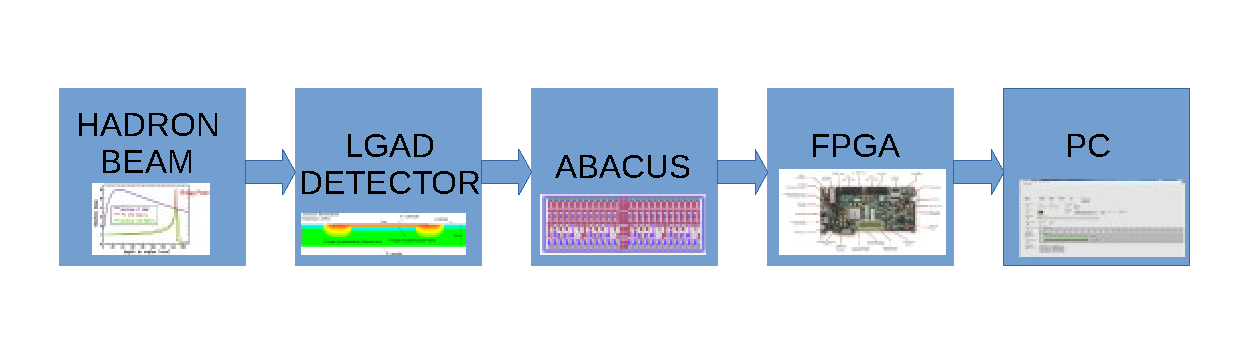
\includegraphics[width=0.99\linewidth]{IMG/ch2/BLOCK}
	\caption{Data flow, from beam to pc}
	\label{fig:block}
\end{figure}
\noindent In figure \ref{fig:block} it can be seen a diagram with the "data flow" of the Project.
The particle beam coming from the accelerators are detected by a LGAD (Low Gain Avalanche Diode) sensor that will be discussed in section \ref{lgad}, the current signal coming from the detector is the digitalized by the second version of a full custom circuit called ABACUS\_v2 that will be discussed in section \ref{chip}.
This ASIC will be mounted on a full custom PCB named EsaAbacus that will be analysed in section \ref{esaabacus}.
The data from the chip is then read by an FPGA board, a general purpose device that will be analysed in detail within chapter 3.
The FPGA elaborates the data and finally sends them to a computer.

\section{MoVe\_IT project}
\begin{figure}[H]
	\centering
	
\includegraphics[width=0.35\linewidth]{IMG/ch2/Move_IT_logo}
	%\caption{}
	%\label{fig:moveit}
\end{figure}
\noindent Currently the Medical Physics group at University of Torino and INFN (the Italian National Institute for
Nuclear and Particle Physics) is participating to the MoVe\_IT\cite{moveit} (Modeling and Verification for Ion beam Treatment planning)
research project, which aims to develop new and
innovative models for biologically optimized Treatment Planning Systems (TPS) using ion beams in hadron therapy.
As~part of the project the Torino group is involved in the development of solid state detectors and readout electronics for measuring with high precision
the characteristics of the hadron beam for irradiation, such as number of particles delivered per unit time, energy and beam profile.
The final goal is to prove the ability of LGAD detectors to discriminate individual protons and to count their number up to fluxes of 100~MHz/cm$^2$ with an uncertainty of less than 1\% which is the clinical tolerance required.
In order to do that a custom detector was built ad hoc for this purpose. It is a LGAD type sensor with an area of $\approx$ 3x3~cm$^2$ and 144 strips. It has a thickness of the active region of 50~$\mu$m.
The final goal is to use two of this sensors in orthogonal directions in order to obtain a greater spatial resolution.
A strip detector is limited in the maximum flux that can be monitored with accuracy, however it is useful in radiobiological experiments, for which it is not needed to reach therapeutic fluxes and often laterally spread-out beams are used\cite{hammad}.
The main key-points of the final design are:
\begin{itemize}
	\item A cover area of $\approx$ 3x3~cm$^2$
	\item A maximum measurable flux of 10$^8$~$\frac{p}{s \cdot cm^2}$ with less than 1\% error
	\item Sensitivity of single particle at low fluxes
	\item Provide beam shape in two orthogonal directions
\end{itemize}


\section{Low Gain Avalanche Diode (LGAD)}\label{lgad}
\noindent The first device involved is the detector. In order to be able to detect a single particle and to reduce the pile-up effects (that have been discussed with great detail in Limardi's masters degree thesis\cite{limardi}) short signals are mandatory. To obtain a short signal the active region of the sensor needs to be the as thin as possible. However the thinner the detector is the lower is the SNR (Signal to Noise Ratio).
To solve this problem the INFN decided to use a new type of sensors known as LGAD.
\noindent Low-Gain Avalanche Detectors (LGADs) are innovative detectors developed in collaboration with the Fondazione Bruno Kessler (FBK, Trento) which feature a moderate ($\approx$10) internal charge multiplication achieved through an additional p+ doping layer few microns depth. The increase signal-to-noise ratio allows designing very thin Ultra Fast Silicon Detectors (UFSD) designed for fast signal collection times, high rates and very good time resolution\cite{lgad}.
%%%%%%%%%%%%%%%%%%%%%%%%%%%%%%%%%%%%%%%%%%%%%%%%%%%%%%%%%%%%%%%%%%%%%%%%%%%%%%%%%%%%%%%%%%%%%%%%%%%%%%%%%%%%%%%%%
The basic doping profiles of the LGAD structure, based on a standard PIN detector, is shown in
figure \ref{fig:ufsdlgad}, showing a n++/p+/p/p++ structure.
The figure shows a highly doped n++ cathode electrode with a moderately doped p+ type region
below, known as the multiplication implant. The n-type electrode has a peak doping concentration
of order 1 $\cdot$ 10$^{19}$ cm$^{-3}$ and has a shallow profile into the bulk of $\approx$ 1 $\mu$m.
The p-type multiplication implant has a peak doping concentration of order 1 $\cdot$ 10$^{16}$ cm$^{-3}$
and has a significantly deeper profile into the bulk ($\approx$ 4 $\mu$m) than the n++ electrode. The bulk
material is high resistivity p-type silicon (approximately 10 k$\Omega$/cm) with a p++ anode electrode
on the backside.
\begin{figure}[H]
	\centering
	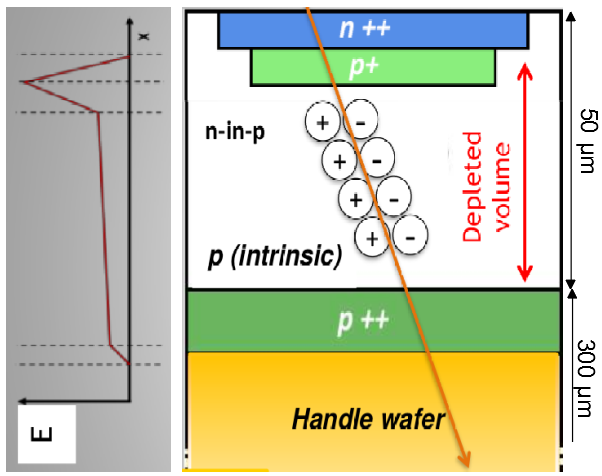
\includegraphics[width=0.35\linewidth]{IMG/ch2/UFSDLGAD.png}
	\caption{Schematic cross-section of the LGAD pad design. A p+ type layer is diffused below the n++ electrode to form the n++/p+/p junction where the multiplication takes place}
	\label{fig:ufsdlgad}
\end{figure}
\noindent The LGAD device is operated with the bulk over depleted. Incident radiation produces electron-hole
pairs in the detector with drift towards the cathode and anode respectively. The maximum
electric field in the device is between the n++ cathode and the p+ type multiplication electrode and is
proportional to the square root of the p+ type doping density and proportional to the square root of the
external bias voltage for an abrupt junction approximation.
The radiation induced electrons in the detector cross this high field region. For sufficiently
high electric fields impact ionisation occurs which results in multiplication of the carriers and a
signal gain.
Increasing the high-field (either due to an increase in the doping density or
an increase in the external bias voltage) will increase the electron-hole pair generation rate. For a
low gain device, the desire is to have an overall gain of 10 at $\approx$~200~V bias, with a breakdown voltage
significantly higher than this at least $\approx$~400~V.
%%%%%%%%%%%%%%%%%%%%%%%%%%%%%%%%%%%%%%%%%%%%%%%%%%%%%%%%%%%%%%%%%%%%%%%%%%%%%%%%%%%%%%%%%%%%%%%%%%%%%%%%%%%%%%%%%
\begin{figure}[H]
	\centering
	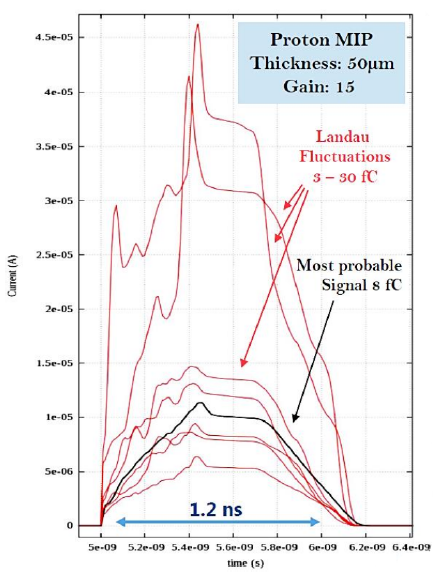
\includegraphics[width=0.35\linewidth]{IMG/ch2/LGAD_Signal}
	\caption{Simulated detector signal}
	\label{fig:signal}
\end{figure}
\noindent The output signal from a detector used in the project has a trapezoidal form, a duration of $\approx$ 1.5~ns and a current in the order of 1$\cdot$10$^{/5}$~A.
In figure \ref{fig:signal} can be seen a signal simulation, the most probable carry a 8~fC charge, however due to the Landau Fluctuations this value can change between 3 and 30~fC.
%%%%%%%%%%%%%%%%%%%%%%%%%%%%%%%%%%%%%%%%%%%%%%%%%%%%%%%%%%%%%%%%%%%%%%%%%%%%%%%%%%%%%%%%%%%%%%%%%%%%%%%%%%%%%%%%%
\noindent The main risk in
the use of LGAD silicon detectors for beam monitoring is related to the high radiation doses from
therapeutic beams. The design of LGAD sensors has not been optimized yet for radiation
resistance, and the measurements performed up to now indicate a stable behavior up to 1014~n$_{eq}$/cm2 for 300~$\mu$m thick detectors (this corresponds to a few hours of a therapeutical proton
pencil beam with an current of 1~nA and a FWHM of $\approx$ 1~cm); at higher doses the internal gain
of the sensors decreases and it is necessary to raise the bias voltage to keep a stable signal level.
It is expected that the use of thinner sensors (50~$\mu$m thickness) will decrease the trapping
probability in the sensors, therefore extending the operative time. Intense work is currently going
on in the LGAD community to increase the radiation resistance of the sensors. Several
approaches as alternative dopants and doping profiles are being investigated with the expectation
to reach a stable behavior up to >1015~n$_{eq}$/cm2 fluencies in the next 1 or 2 years.


\section{ABACUS chip}\label{chip}
\noindent The signal from figure \ref{fig:signal} of each detector strip is connected to an input channel of the new ABACUS\_v2 full custom chip\cite{abacus}\cite{dac}.
\begin{figure}[H]
	\centering
	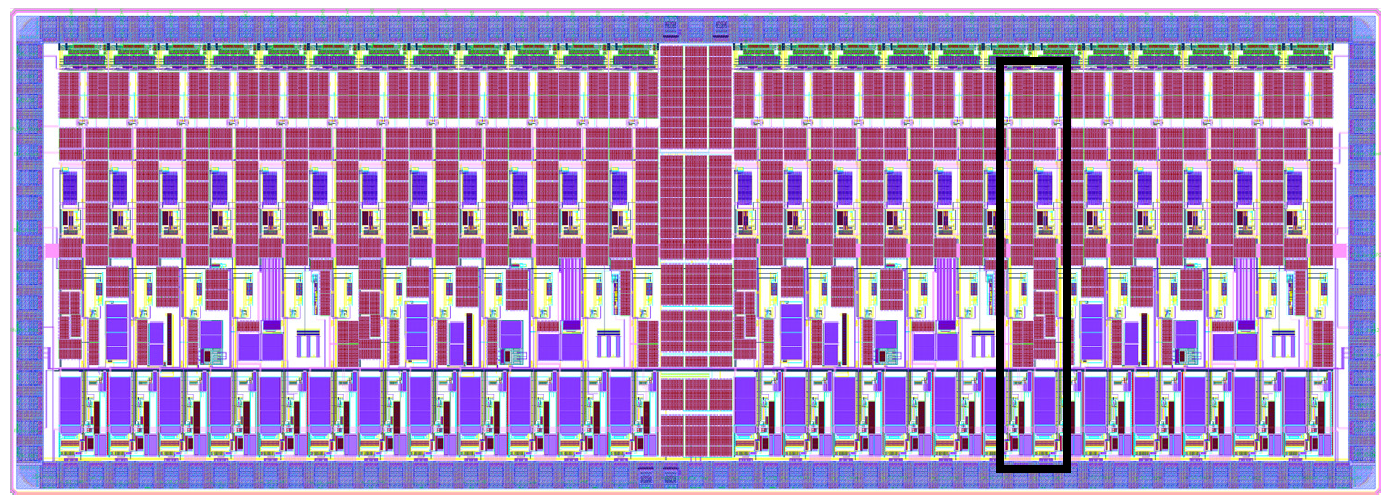
\includegraphics[width=0.9\linewidth]{IMG/ch2/ABACUS2.png}
	\caption{ABACUS\_v2 chip die view}
	\label{fig:abacus2}
\end{figure}

\begin{figure}[H]
	\centering
	\includegraphics[width=0.8\linewidth]{IMG/ch2/Abacus_channel.png}
	\caption{Single channel diagram of the ABACUS\_v2 chip}
	\label{fig:abacuschannel}
\end{figure}

\section{Esa-Abacus}\label{esaabacus}
\begin{figure}[H]
	\centering
	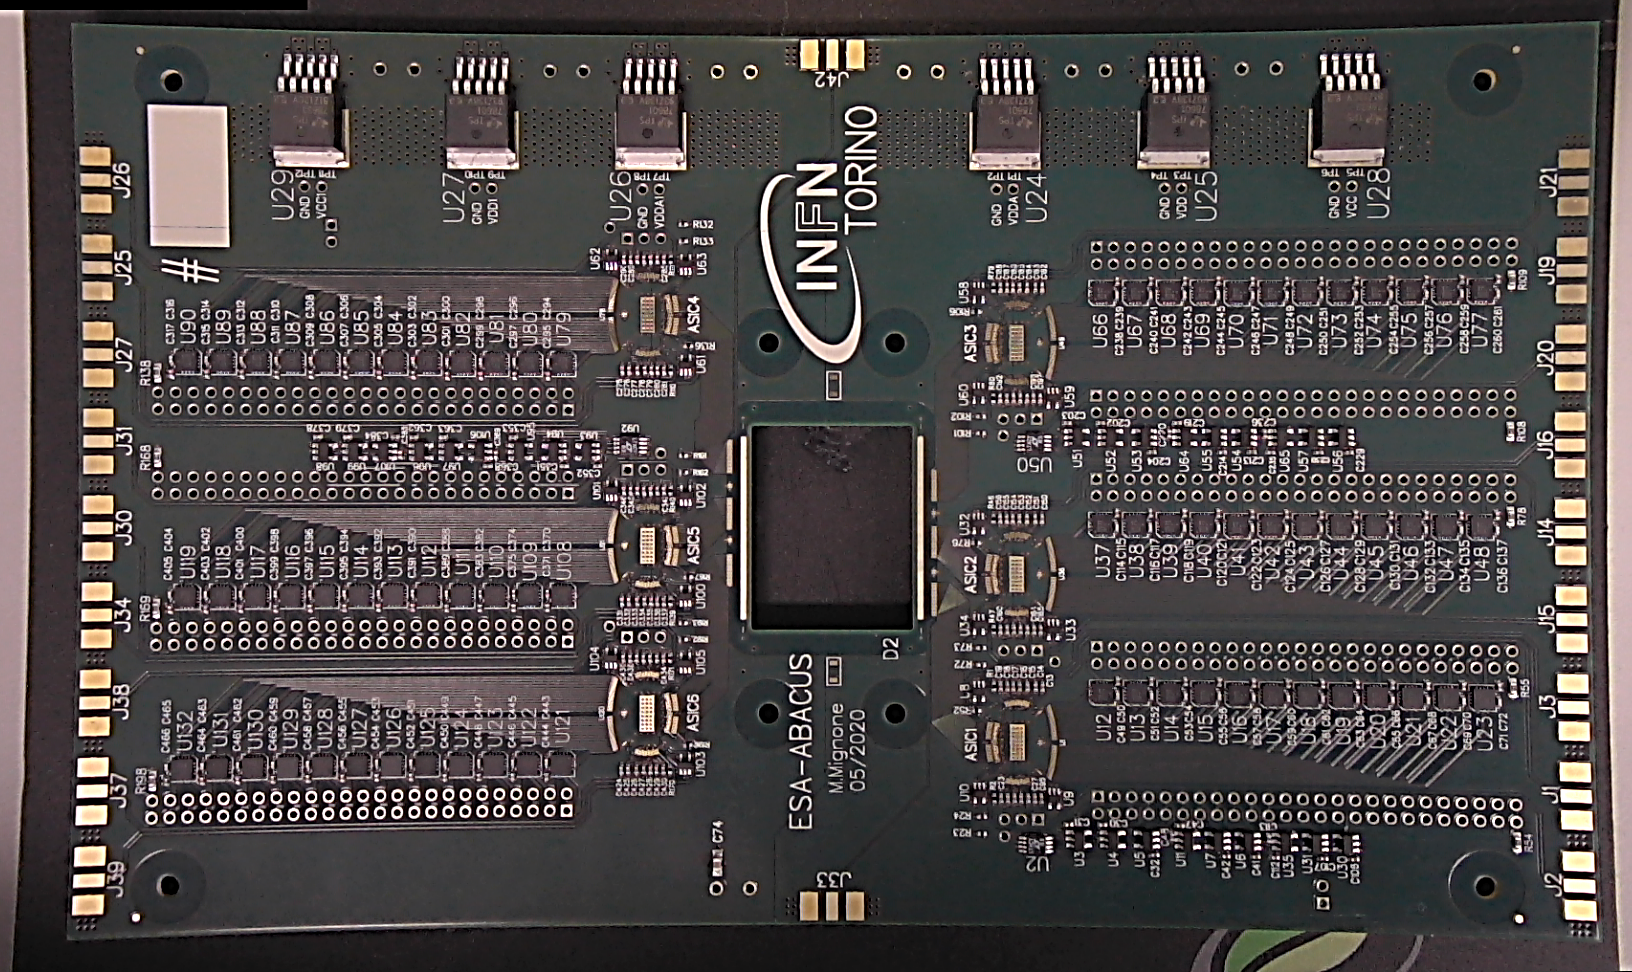
\includegraphics[width=0.7\linewidth]{IMG/ch2/EsaAbacus.png}
	\caption{Esa-Abacus board}
	\label{fig:esaabacus}
\end{figure}

\section{FPGA board}

%\section{Beam test with strip sensor}
%\section{Verification of counting skills}